% pipeline-vE — hand-authored TikZ figure (absolute coordinates; no auto-layout).
% Build:  bash docs/figures/build.sh pipeline-vE     (CAPTION=1 for the paper build)
%
% Variant E of docs/figures/pipeline.tex. Palette, box geometry, arrow idioms, the note/lbl
% styles and the caption switch are unchanged from that file, which takes them in turn from
% trec-ragtime-2026/docs/figures/pipeline.tex, so a change to the house style belongs in all
% three.
%
% THE ONE IDEA, unchanged: two bands, one above the other, and the white gap between them is the
% interface. Everything the model decides sits in the upper band; everything that adjudicates and
% remembers sits in the lower one. Every arrow that crosses the gap carries a label, because the
% crossing is the only place where authority changes hands and the reader must be told what
% travels. Nothing else is labelled: inside a band the arrows are mechanical.
%
% WHAT VARIANT E ADDS: the trace, drawn as its two halves. The original drew only the record, the
% orchestrator's account, as a slab across the lower band. A pass also writes a TRANSCRIPT, the
% conversation the model reads, and the taxonomy the paper has just introduced makes the two
% halves of one object. So the transcript is drawn the same way the record is -- a wide slab in
% the mod style, a bold name over one \sublabel line of $\cdot$-separated contents, the same 10mm
% height -- but in the MODEL's band, because the transcript is what the model reads and it is the
% model's half. Ownership is the reason it could not simply be parked beside the record.
%
% CEILING, unchanged: no thresholds, no constants, no code identifiers. The drawing says who
% decides what, not with which numbers.
%
% HEIGHT is the budget. The figure runs at full text width in a two-column paper, so its height
% is what costs page space; width is nearly free, since a wider figure is scaled down further to
% reach \textwidth and so occupies LESS page height. Variant E therefore pays for the transcript
% in width, not in height, and finishes shorter than the original.
%
% DEPARTURES FROM THE ORIGINAL, each overruling a comment that is quoted where it is overruled:
%   1. The question enters from the LEFT, not from above.        (see THE QUESTION)
%   2. The band title and its note share one line.               (see BAND TITLES)
%   3. The rail is gone; the transcript's lower edge replaces it.(see THE MENU)
%   4. Each tool now has a returning arrow as well as a call.    (see THE FOUR TOOLS)
%   5. The record's sub-label loses "the answers tried".         (see THE TRACE)
% varwidth is raised from 210mm to 230mm: the figure is deliberately wider than the original and
% would otherwise be wrapped by the standalone class rather than measured.
\documentclass[border=8pt,varwidth=230mm]{standalone}
\usepackage{tikz}
\usetikzlibrary{shapes.geometric,arrows.meta,calc,backgrounds}

\definecolor{bluevar}{HTML}{2F6BC0}
\definecolor{ambervar}{HTML}{C5701F}
\definecolor{greenvar}{HTML}{1B7A3E}
\definecolor{slatefill}{HTML}{E9EDF2}
\definecolor{slatestroke}{HTML}{4A5563}
\definecolor{modstroke}{HTML}{33404F}
\definecolor{loopstroke}{HTML}{555F6B}
% tracefill is the ONE thing in this drawing that two boxes share and no other box has, and it
% is what ties the transcript to the record as ink rather than as a claim in a note. It is not a
% new hue: it is the slate family carried two steps past slatefill, so the figure stays
% monochrome and the tint survives greyscale printing. The value is chosen for the WORSE of its
% two backgrounds -- the record sits on the full-strength orchestrator band, the transcript on
% the 45%% one -- so that the darker case still separates. Luminances: white boxes 255, model
% band 247, gates 240, orchestrator band 236, tracefill 217. It is the darkest fill in the
% picture, which is right: the two slabs are the two things the pass actually leaves behind.
\definecolor{tracefill}{HTML}{D3DAE4}

% Caption switch, same name and default in every figure source here. The caption is drawn inside
% the exported image and the README carries that text in its own prose, so it is off unless the
% build defines \withcaption:  CAPTION=1 bash docs/figures/build.sh pipeline-vE.
\newif\ifshowcaption
\showcaptionfalse
\ifdefined\withcaption\showcaptiontrue\fi

\newcommand{\sublabel}{\fontsize{6.5}{7.5}\selectfont}
\begin{document}
\centering
% No hyphenation inside the drawing: a label broken as "en-tailment" reads as a typo, and every
% label here is short enough to wrap on a word. The group keeps this local to the picture so the
% caption below still hyphenates normally.
{\hyphenpenalty=10000 \exhyphenpenalty=10000 \tolerance=9999 \emergencystretch=2em
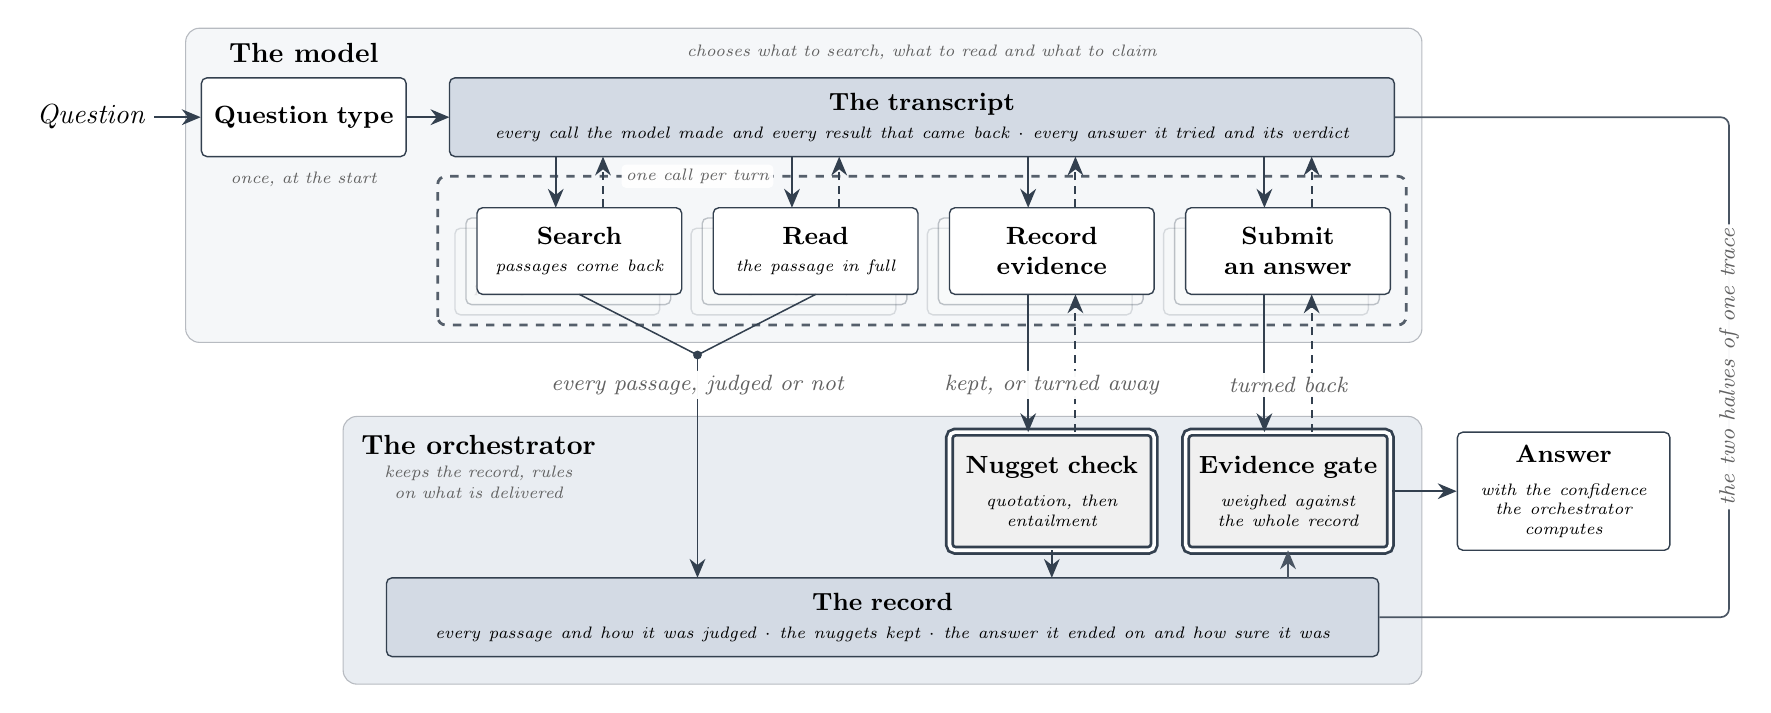
\begin{tikzpicture}[
  >={Stealth[length=2.4mm,width=2mm]},
  font=\small,
  mod/.style={draw=modstroke,line width=0.5pt,fill=white,rounded corners=2pt,
              align=center,minimum width=38mm,minimum height=10mm,inner sep=2pt},
  flow/.style={draw=modstroke,line width=0.7pt,->},
  fan/.style={draw=modstroke,line width=0.55pt,->},
  runedge/.style={draw=slatestroke,line width=0.6pt,->,densely dashed},
  % The record is READ, not written, by the answer gate. Giving that one arrow the softer slate
  % stroke is what stops the reader taking it for another write.
  readedge/.style={draw=slatestroke,line width=0.7pt,->},
  gate/.style={draw=modstroke,line width=1pt,double,double distance=1.3pt,fill=black!6,
               rounded corners=2pt,align=center,inner sep=2pt},
  % THE TIE. The transcript and the record are the two halves of one trace, and until now the
  % figure said so only by position, by their shared 10mm height and label form, and by one
  % sentence in the gap. A reader who did not read the sentence saw two unrelated boxes. slab is
  % mod with the shared fill, and it is applied to those two nodes and to nothing else, so the
  % pairing is carried by ink.
  % WHY A FILL AND NOT A LINE. A connector was measured and is not available. Sweeping x from
  % -1.0 to 20.0, the only straight vertical corridors between the transcript's underside (8.70)
  % and the record's top (3.35) that clear every rule, box, ghost, arrow and label by 0.10 are
  % OUTSIDE both bands, at x <= -0.15 and x >= 19.0, and neither slab has an edge there. The
  % transcript cannot be left westward, because Question type occupies x 0.20..2.80 over exactly
  % its own y span of 8.70..9.70; it cannot be left southward, because the enclosure's top rule
  % runs the slab's full width 0.25 beneath it. Every remaining route needs a dogleg through the
  % tool row's gutters, which the piled ghosts fill, or a crossing of the answer's exit arrow.
  % A fill also survives what a hairline may not: at the 0.788 print scale a 0.4pt tie rule
  % becomes 0.32pt, while an area of tint is scale-free. And a fill cannot be misread as traffic,
  % which a fifth line in a figure with three arrow idioms certainly would be.
  % WHY IT RESPECTS OWNERSHIP. The tie is a property the two slabs both have, not a mark drawn
  % from one band into the other. Nothing crosses the gap, so neither actor reaches into the
  % other's territory to claim the pairing.
  slab/.style={mod,fill=tracefill},
  % THE BRACKET. Headless, so it cannot be read as traffic: every arrow in this figure carries a
  % head and this carries none. Slate rather than modstroke, the same softer stroke the readedge
  % uses, because it is not a step either. Rounded corners match the bands' own 5pt idiom.
  tie/.style={draw=slatestroke,line width=0.6pt,rounded corners=3pt},
  % NOTE ON text width, which every node with a title carries -- the boxes, the two slabs and the
  % band notes -- and no lbl does. It is not there to
  % break lines -- every break in this figure is an explicit \\ -- it is there for the interword
  % space. A node without it sets each line at the natural space of whatever font is current, so
  % a \bfseries title spaces wider than its \sublabel sub-label and the two read as different
  % typography. With text width the node becomes a real paragraph, \emergencystretch above takes
  % the slack, and every space in the picture settles at one value per node size. Keep it below
  % the box's minimum width (the node is as wide as max(minimum width, text width + 2*inner sep))
  % or the box grows to fit it.
  note/.style={font=\sublabel\itshape,text=black!62,align=center},
  % white backing so a label stays legible over the arrow it names; font in OPTIONS (not inline)
  % so the WHOLE multi-line label is styled, not just its first line:
  lbl/.style={fill=white,fill opacity=0.97,text opacity=1,inner sep=1.5pt,rounded corners=1.5pt,
              font=\footnotesize\itshape,text=black!62,align=center},
]

% ================= THE TWO BANDS =============================================================
% Drawn first, so everything else lands on top of them; no background layer is needed and the
% draw order stays readable. Both bands stop at x = 15.7 and share the same 5pt corner radius, so
% the eye reads them as one column split in two rather than as two unrelated panels. The model's
% band starts further left (0.0 against 2.0): it has to hold the typing step as well as the four
% tools, and that left overhang is now the INTAKE SIDE -- the question crosses the band's LEFT
% border to reach it, where in the original it crossed the top border.
%
% VERTICAL EXTENTS ARE STILL MEASURED, NOT CHOSEN, and everything from the tool row downwards is
% the original's geometry untouched: the model band's floor is 6.34 because the lowest ink inside
% it is the faintest piled copy at 6.69, the dashed enclosure clears that by 0.13 at 6.56, and
% the band clears the enclosure by 0.22; the merge dot sits 0.16 BELOW the border, in the gap,
% because there is no longer room for it between the enclosure and the floor. The orchestrator
% band is unchanged at 2.00..5.40.
% What changed is the model band's CEILING, 9.80 -> 10.33, and the arithmetic that pays for the
% transcript is worth writing down because nothing else in the figure had any slack. The slab is
% 1.00 tall and the lane beneath it is 0.65 where the old rail's droppers needed 0.45, so the
% bill is 1.20. It was met in four places and there were no others. 0.53 by raising the band's
% ceiling into the strip that the question's label and its arrow used to occupy OUTSIDE the band
% (9.80 up to 10.38), which entering from the left gives back for nothing. 0.31 by setting the
% band title and its note on one line instead of two, collapsing a 0.94 title row to 0.63. 0.10
% by taking the tool boxes from 12mm to 11mm, which still leaves them 1mm of air above and below
% their two lines. And 0.26 from the rail itself, which no longer exists because the slab's lower
% edge is now the thing the fan hangs from. Measured: 252.465 x 607.403pt against the original's
% 253.545 x 550.719, so the drawing is 1.1pt SHORTER and 56.7pt wider, and at \textwidth the
% extra width scales it shorter again.
%
% The upper band is tinted at slatefill!45 and the lower at full slatefill. The model band has to
% stay the lighter of the two because it holds four white boxes and a white slab and would
% otherwise swallow them; the orchestrator band holds the grey gates and the record, and takes
% the stronger tint so that the gap between the bands -- the interface -- is the brightest
% horizontal stripe in the figure.
\fill[slatefill!45,rounded corners=5pt] (0.0,6.34) rectangle (15.7,10.33);
\draw[slatestroke!40,line width=0.4pt,rounded corners=5pt] (0.0,6.34) rectangle (15.7,10.33);
\fill[slatefill,rounded corners=5pt] (2.0,2.00) rectangle (15.7,5.40);
\draw[slatestroke!40,line width=0.4pt,rounded corners=5pt] (2.0,2.00) rectangle (15.7,5.40);

% ================= BAND TITLES ===============================================================
% font=\bfseries (not {\bfseries ...} inside the node) deliberately overrides the picture's
% font=\small, so the two band names are the largest type in the drawing and rank above every box
% title.
% DEPARTURE 2. Overruled: "The model's title stays at x = 9.5. That is no longer the centre of
% the widened band, but it is the centre of what is left of the band once Question type has taken
% the left overhang". Two things void that reasoning. The centred title occupied a full 0.94-unit
% row (8.86..9.80) that the transcript now needs, and the orchestrator's title sits at ITS band's
% left margin, so a centred model title was the odd one out. The model's title moves to the same
% left margin, its note stays where it always was, centred on the band's content, and the two
% simply share a line. The note gains a second job there: it now sits directly over the
% transcript slab and reads as a header for the band and for the slab at once.
\node[font=\bfseries] at (1.50,10.02) {The model};
\node[note,text width=80mm] at (9.35,10.02) {chooses what to search, what to read and what to claim};
% x = 3.72, not 4.95, for the reason the original gives: at 4.95 the title's right edge reached
% 6.44 against the long vertical arrow at 6.50, a 1.7pt miss that read as a collision. Unchanged.
\node[font=\bfseries] at (3.72,5.04) {The orchestrator};
% Two lines, so its top sits higher above the node centre than a one-line note would; 4.68 put it
% against the title's descenders.
\node[note,text width=36mm] at (3.72,4.56) {keeps the record, rules\\on what is delivered};

% ================= THE QUESTION AND ITS TYPE =================================================
% Question type sits INSIDE the model band: the model is what assigns the type, so drawing it
% outside a band titled "The model" contradicts the band. It goes in the band's left overhang
% rather than in the tool row, and it is the one box in the band with no pile behind it and no
% dashed enclosure around it -- that is how the drawing says it fires once. The note under it
% says so in words afterwards.
%
% DEPARTURE 1. Overruled: "The italic 'Question' stays OUTSIDE the band, because the question is
% the one thing here that really does arrive from elsewhere; its arrow crosses the band's top
% border to say so." The reasoning survives intact and only the border changes: the question is
% still outside the band, and its arrow still crosses a band border to get in. Entering from the
% LEFT buys two things the top entry could not. It returns the 0.54 units the label and its arrow
% held above the band, which is most of what the transcript costs. And it makes the figure read
% straight across: the question comes in through the left wall of the upper band and the answer
% leaves through the right wall of the lower band, so the two things that cross the outside of
% the drawing are now a matched pair on the same axis instead of one entering downwards and one
% leaving sideways. "Question" sits to the left of its arrow on the arrow's own line, exactly as
% "Answer" sits to the right of its arrow on its line.
\node[align=center,font=\itshape,anchor=east] (question) at (-0.40,9.20) {Question};
% The box is 10mm high, the mod default -- the same height as the transcript slab it hands to,
% and shorter than the 11mm menu boxes, so it does not read as a fifth tool that has wandered off
% to the left. It is set at the slab's own centre line so the hand-off is one straight horizontal
% arrow with no dogleg, the rule the gates below are already drawn by.
\node[mod,text width=24mm,minimum width=26mm] (type) at (1.50,9.20) {\bfseries Question type};
\node[note,text width=26mm] at (1.50,8.41) {once, at the start};
\draw[flow] (question) -- (type);
% The type is put in front of the model by being written into the transcript, which is why this
% arrow ends on the slab and not on the tool row. It also keeps the type outside the dashed
% enclosure without needing to cross it.
\draw[flow] (type.east) -- (3.35,9.20);

% ================= THE TRACE, HALF ONE: THE TRANSCRIPT =======================================
% DEPARTURE 5 lives here and in the record below. The original record slab read "every passage
% retrieved and how it was judged $\cdot$ the nuggets kept $\cdot$ the answers tried". Under the
% taxonomy the answers tried are not the orchestrator's account of the pass, they are the
% conversation, so they move up here and the record takes in their place the thing it alone
% holds, the answer the pass finished on together with how sure it was.
%
% The slab is the model's, and it is drawn in the model's band, because the transcript is what
% the model reads. It is deliberately the same object as the record: same mod style, same 10mm
% height, same bold name over one \sublabel line of $\cdot$-separated contents, both spanning
% nearly the whole width of the band they belong to. The two are the same shape on opposite sides
% of the interface, which is what "two halves" has to look like before any label says it. They
% cannot be the same WIDTH -- the model's band has a left overhang the orchestrator's does not,
% and the slab has to leave room for Question type -- so height and idiom carry the rhyme.
%
% It sits ABOVE the dashed enclosure, not inside it, and that is load-bearing: the enclosure is
% what repeats, and the transcript does not. It is one growing surface that every turn reads from
% and appends to, so it belongs outside the repeating region exactly as Question type does.
\node[slab,text width=118mm,minimum width=120mm] (script) at (9.35,9.20)
   {{\bfseries The transcript}\\[-1pt]{\sublabel\itshape every call the model made and every result that came back $\cdot$ every answer it tried and its verdict}};

% ================= THE MENU, AND THE FACT THAT IT REPEATS ====================================
% The pile idiom is trec-ragtime-2026's: one \newcommand holding the repeatable content, called
% at two offsets with opacity 0.30 and 0.16 BEFORE the front copy, so the faded copies land
% behind everything drawn later. Ours pile the four boxes ONLY, where the reference piles the
% dashed enclosure with them. That is forced, not preferred: our enclosure is nearly as wide as
% the band, so a piled frame puts a ghost right rule on the Submit box's own edge. Piling the
% boxes inside a single frame says the same thing -- this row happens again and again -- and says
% it without a second set of rules to read.
% The offsets are down-and-left because the boxes shift into their own 0.4 gutters that way, and
% because up or right would run the ghosts under the droppers or off the band.
% KEEP IN SYNC with the front row below: same four boxes, same coordinates, same text.
\newcommand{\menucontent}[3]{% #1=dx  #2=dy  #3=opacity
  \begin{scope}[shift={(#1,#2)},opacity=#3]
    \node[mod,text width=24mm,minimum width=26mm,minimum height=11mm] at (5.0,7.50)
       {{\bfseries Search}\\[-1pt]{\sublabel\itshape passages come back}};
    \node[mod,text width=24mm,minimum width=26mm,minimum height=11mm] at (8.0,7.50)
       {{\bfseries Read}\\[-1pt]{\sublabel\itshape the passage in full}};
    \node[mod,text width=24mm,minimum width=26mm,minimum height=11mm] at (11.0,7.50)
       {{\bfseries Record}\\{\bfseries evidence}};
    \node[mod,text width=24mm,minimum width=26mm,minimum height=11mm] at (14.0,7.50)
       {{\bfseries Submit}\\{\bfseries an answer}};
  \end{scope}}
\menucontent{-0.28}{-0.26}{0.16}
\menucontent{-0.14}{-0.13}{0.30}

% The enclosure. Dashed, in loopstroke, the house colour for "this region iterates". It holds the
% four boxes and the arrows that reach them, and nothing else, so its boundary is exactly the
% line that Question type and the transcript are both drawn outside of. Padding is 0.5 on the
% left and 0.2 on the right because the piled copies eat the left gutter; the top hangs 0.25
% under the slab and 0.40 above the tool boxes, which is what leaves the lane wide enough for a
% pair of arrows and a label; the bottom clears the lowest ghost (6.69) by 0.13.
\draw[dashed,draw=loopstroke,line width=1pt,rounded corners=3pt] (3.20,6.56) rectangle (15.50,8.45);

% ================= THE FOUR TOOLS ============================================================
% All four at the same height, evenly pitched at 3.0 with 2.6 of box, so the 0.4 gutters read as
% deliberate. Equal height is the whole point: the model may reach for any of them on any turn,
% and any vertical stagger would draw an order that does not exist. They are a MENU picked from
% one at a time, which the pile behind each box and the "one call per turn" label both say.
% 11mm tall, not the original 12: two lines and their inner sep need 9.0mm, so 1mm of air
% survives above and below, and the millimetre given up here is a millimetre the lane between the
% slab and the boxes gets instead, where two arrows now have to fit rather than one.
% A sub-label is closed off in its OWN group per line, rather than written as one
% {\sublabel\itshape a\\b}. The break then happens while the node font is still \small, so the
% leading is 11pt and the \\[-1pt] under a title lands on 11pt too; wrap the whole sub-label in
% one group instead and the title-to-sub gap collapses and the sub-label crowds its title. The
% two-line bold titles repeat \bfseries for the same reason of symmetry.
% The two right-hand boxes carry a two-line TITLE and no sub-label. They are the two tools whose
% names already say what they do, and a sub-label under them would have collided with the gate
% arrows leaving their south edges.
\node[mod,text width=24mm,minimum width=26mm,minimum height=11mm] (search) at (5.0,7.50)
   {{\bfseries Search}\\[-1pt]{\sublabel\itshape passages come back}};
\node[mod,text width=24mm,minimum width=26mm,minimum height=11mm] (read) at (8.0,7.50)
   {{\bfseries Read}\\[-1pt]{\sublabel\itshape the passage in full}};
\node[mod,text width=24mm,minimum width=26mm,minimum height=11mm] (rec) at (11.0,7.50)
   {{\bfseries Record}\\{\bfseries evidence}};
\node[mod,text width=24mm,minimum width=26mm,minimum height=11mm] (submit) at (14.0,7.50)
   {{\bfseries Submit}\\{\bfseries an answer}};

% DEPARTURES 3 AND 4. Overruled: "The rail: one horizontal line above the four boxes, dropping a
% head into each. This is the agentic recurrence drawn as a fan rather than as a cycle -- a chain
% search->read->record->submit would assert an order the loop does not enforce." The fan is kept
% and so is the reason for it; what goes is the bare horizontal line the fan used to hang from.
% It was an unnamed bus, and the drawing now has the named thing that the fan actually comes out
% of: the model reads the transcript and makes one call. The slab's lower edge is the rail, the
% four droppers leave it, and the junction dot that used to mark where the question's line became
% the menu is no longer needed, because the type's line ends in the slab instead.
% The second arrow of each pair is the departure the transcript forces. A tool call and the
% result that comes back are BOTH conversation, so both have to reach the slab, and the figure
% already has an idiom for exactly that: the gates below are drawn as a solid request down the
% left of the box and a dashed reply up its right, at the same 3mm offset. Reusing it here means
% the pairs need no label of their own, and it lines up: at x = 10.7 and 13.7 a single straight
% solid line now runs from the transcript through the tool to the gate, and at 11.3 and 14.3 the
% dashed reply runs all the way back, so the reader sees one round trip rather than three hops.
\foreach \x in {5.0,8.0,11.0,14.0}{
  \draw[flow] (\x-0.3,8.70) -- (\x-0.3,8.05);
  \draw[flow,densely dashed] (\x+0.3,8.05) -- (\x+0.3,8.70);
}
% Sits in the lane between the slab and the boxes, in the clear 2.4 units between the Search pair
% and the Read pair, on the same x = 6.5 axis as the merge dot and its label below, so the three
% left-hand annotations of the figure share one vertical line. It is set ON the enclosure's top
% rule and drawn after it, so the white backing punches through the dashed line -- the same trick
% the original played with the rail, and apt here for a different reason: the sentence is about
% what crosses into the repeating region, so it straddles that region's boundary. It also leaves
% the label the full 0.65 of the lane instead of half of it, which is the only way it fits with
% clearance above and below.
\node[lbl,font=\sublabel\itshape] at (6.5,8.45) {one call per turn};

% ================= SEARCH AND READ FEED THE RECORD ===========================================
% Both retrieval tools write to the record whether or not the model goes on to use what came
% back, so the two lines MERGE at a dot and cross the gap as one arrow. Two parallel arrows would
% have suggested two separate deposits and needed the same label twice.
% The dot is at 6.18, i.e. 0.16 BELOW the model band's floor rather than inside it. The floor
% hugs the piled copies and there is no room between the enclosure (6.56) and the band (6.34) for
% a dot with clearance on both sides, and a dot 1pt off a dashed rule looks like a mistake. In
% the gap it has 0.10 to the border above and 0.11 to its label below.
\draw[fan,-] (5.0,6.95) -- (6.5,6.18);
\draw[fan,-] (8.0,6.95) -- (6.5,6.18);
\fill[modstroke] (6.5,6.18) circle[radius=1.6pt];
\draw[flow] (6.5,6.18) -- (6.5,3.35);

% ================= THE TWO GATES =============================================================
% Deliberately aligned to the same x as the two tools they adjudicate, so each solid/dashed pair
% is a straight vertical drop with no dogleg -- and now that the tools carry the same pair above
% them, that drop runs the whole height of the figure. The double rule and the grey fill are the
% house idiom for "code decides here", carried over from the companion figure's verbatim check.
% Their tops sit 0.20 under their band's ceiling, the same margin the band gives the record
% below. 15mm tall, not 16: three lines and their inner sep need 13.6mm.
\node[gate,text width=24mm,minimum width=26mm,minimum height=15mm] (ngate) at (11.0,4.45)
   {{\bfseries Nugget check}\\[1pt]{\sublabel\itshape quotation, then}\\[-4pt]{\sublabel\itshape entailment}};
\node[gate,text width=24mm,minimum width=26mm,minimum height=15mm] (agate) at (14.0,4.45)
   {{\bfseries Evidence gate}\\[1pt]{\sublabel\itshape weighed against}\\[-4pt]{\sublabel\itshape the whole record}};

% Each pair is offset 3mm either side of the box centre: the request goes down solid on the left,
% the verdict comes back dashed on the right. 3mm is the smallest offset that still leaves the
% two mid-gap labels room to sit between the pairs without their backings touching.
\draw[flow] (10.7,6.95) -- (10.7,5.20);
\draw[flow,densely dashed] (11.3,5.20) -- (11.3,6.95);
\draw[flow] (13.7,6.95) -- (13.7,5.20);
\draw[flow,densely dashed] (14.3,5.20) -- (14.3,6.95);

% The three labels of the crossing, all on y = 5.80. Keeping them on one line makes the gap read
% as a single boundary rather than as three unrelated hops. They are not on the gap's midline:
% the merge dot sits in the gap too, so the row was set 0.185 above the lower band's ceiling and
% what is left over goes above it, to the dot. The gap is 0.94 (6.34 down to 5.40); the labels
% are 0.43 tall, which is what fixes it.
\node[lbl] at (6.5,5.80) {every passage, judged or not};
\node[lbl] at (11.0,5.80) {kept, or turned away};
\node[lbl] at (14.0,5.80) {turned back};

% ================= WHERE THE WORD "TRACE" GOES ===============================================
% One sentence, and it is put in the GAP, at the left, on the same row as the three crossing
% labels. That is the only region of the drawing that belongs to neither band, and this is the
% only statement in the drawing that is about both bands at once -- everything else in the figure
% is owned, and the two halves it names are owned by different actors, so it cannot sit in either
% band without taking a side. Putting it on the crossing row is the second half of the argument:
% the reader is already reading that row to learn what the interface is, and this is the same
% kind of fact. It is set in the \sublabel note style rather than the larger lbl of its
% neighbours because it is not labelling an arrow; it is the caption of a relationship, which is
% what the band notes are too.
% The left end of "every passage, judged or not" is at 4.53, so 40mm centred on 2.30 clears it by
% 0.23; two lines at 6.5pt are 0.53 tall inside a 0.94 gap.
% The note that used to sit here is gone: the bracket at the right now names the trace, on the
% line that draws it, so a sentence in the gap would say the same thing twice.

% ================= THE TRACE, HALF TWO: THE RECORD ===========================================
% A slab, not a box: it spans almost the whole orchestrator band because everything above it
% writes to it. Drawn after the arrows that end on its top edge, so its white fill trims them
% cleanly. It keeps 0.55 of band on either side, so it still reads as the floor of the band
% rather than as a box parked in it. 10mm tall, matching the transcript exactly, which is one of
% the three things that make the two read as one object; two lines and their inner sep need
% 9.0mm, and every millimetre here is a millimetre of page. Its top stays 0.35 under the gates --
% the two arrows that meet it are short by design, they only have to say which way the traffic
% goes -- and the 1mm it gives up against the original goes to its clearance from the band floor.
% See DEPARTURE 5 at the transcript above for why "the answers tried" is no longer here.
\node[slab,text width=124mm,minimum width=126mm] (record) at (8.85,2.85)
   {{\bfseries The record}\\[-1pt]{\sublabel\itshape every passage and how it was judged $\cdot$ the nuggets kept $\cdot$ the answer it ended on and how sure it was}};
\draw[flow] (11.0,3.7) -- (11.0,3.35);
% The only upward arrow into a slab in this band, and the only readedge: the answer gate consults
% the record it does not write. Different colour, same weight, opposite direction -- three cues,
% because a reader who takes this for a write misreads the whole lower band.
\draw[readedge] (14.0,3.35) -- (14.0,3.7);

% ================= WHAT LEAVES ===============================================================
% Outside the bands, mirroring the question on the left: the answer is what the orchestrator
% hands back, so it leaves the orchestrator band sideways, and the question now enters the model
% band sideways too, on the same reading axis. Same height and same box metrics as the gates, so
% the exit reads as one straight line out of the Evidence gate.
\node[mod,text width=25mm,minimum width=27mm,minimum height=15mm] (answer) at (17.5,4.45)
   {{\bfseries Answer}\\[1pt]{\sublabel\itshape with the confidence}\\[-4pt]{\sublabel\itshape the orchestrator}\\[-4pt]{\sublabel\itshape computes}};
\draw[flow] (agate.east) -- (answer.west);


% ================= THE BRACKET THAT NAMES THE TRACE ==========================================
% A ] on its side, from the record's east edge out past the Answer box, up the right margin and
% back into the transcript's east edge. It runs at y = 2.85, which is BELOW the Answer box's floor
% at 3.70, so it passes under the box and the box stays readable. The vertical leg sits at 19.60,
% 0.75 clear of the Answer box's right edge at 18.85, in white space that belongs to neither band
% -- which is the point, since the trace belongs to neither actor. The label rides the middle of
% that leg, rotated so the bracket costs width and not height, with the same white backing the
% rail's "one call per turn" uses, punched through the line it names.
\draw[tie] (record.east) -- (19.60,2.85) -- (19.60,9.20) -- (script.east);
\node[lbl,rotate=90] at (19.60,6.03) {the two halves of one trace};

\end{tikzpicture}}

\ifshowcaption
\vspace{10pt}
\parbox{188mm}{\footnotesize One question through the pipeline, where the model chooses what to
search, read and claim and the orchestrator keeps the record and rules on what is delivered. The
transcript and the record are the two halves of the trace one pass leaves behind.}
\fi
\end{document}
